\documentclass[tikz, border=3mm]{standalone}
\usepackage{tikz}
\usetikzlibrary{arrows.meta, calc, angles, quotes, positioning}

\begin{document}
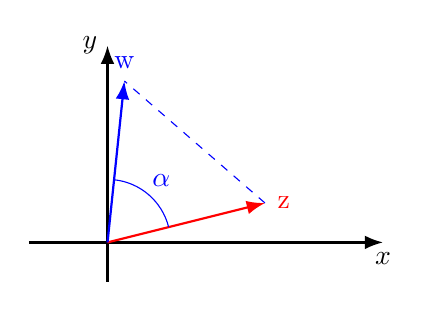
\begin{tikzpicture}[
    >=Latex, % Set default arrow tip style
    vector/.style={->, thick} % Style for vectors
]

    % --- Definitions ---
    \coordinate (origin) at (0,0);
    \coordinate (z_end) at (2, 0.5); % Endpoint of vector z
    \def\alphaa{70} % Rotation angle in degrees (adjust as needed)

    % --- Calculations ---
    % Calculate endpoint of w by rotating z_end around origin by alpha
    % Use let..in to get length (n1) and angle (n2) of z
    \path let \p1=(z_end), \n1={veclen(\x1,\y1)}, \n2={atan2(\y1,\x1)} in
        % Define w_end using the same length (n1) and rotated angle (n2+alpha)
        coordinate (w_end) at ({\n2+\alphaa}:\n1); % Polar coords: angle:radius

    % --- Drawing ---
    % Axes (adjust limits if needed based on rotation)
    \draw[->, thick] (-1, 0) -- (3.5, 0) node[below] {$x$};
    \draw[->, thick] (0, -0.5) -- (0, 2.5) node[left] {$y$};

    % Draw Red Vector 'z'
    \draw[vector, red] (origin) -- (z_end);
    \node[red, right=1pt of z_end] {z}; % Label near endpoint

    % Draw Blue Vector 'w' (the rotated vector)
    \draw[vector, blue] (origin) -- (w_end);
    \node[blue, above=1pt of w_end] {w}; % Label near endpoint

    % Draw Dashed line representing the vector w-z (connecting endpoints)
    \draw[dashed, blue] (z_end) -- (w_end);

    % Draw Angle Arc 'alpha' between z and w
    \pic [draw, blue, angle radius=0.8cm, "$\alpha$", angle eccentricity=1.3] {angle = z_end--origin--w_end}; % Angle at origin

\end{tikzpicture}
\end{document}